\chapter{Appendix}

\section{\#42 Public Transport in the UK}


\subsection*{Rationale for Excluding Transport Lines and Year Data}
The decision to exclude transport lines and year data from the network files was based on several considerations. Firstly, the primary focus of this study was to analyze the structural properties of the transport networks within the UK. Including detailed line information and historical data would have added complexity without significantly enhancing the analysis of network topology and connectivity.

The datasets available were limited to one week of data, as detailed in the original paper by Gallotti et al. (2015)\cite{gallotti2015}, making it impossible to include the year data. Furthermore, differentiating the network for each day of the week was deemed uninteresting for the scope of this study.

The temporal data file provided contained events, essentially the timetable of stops. Handling this file was challenging due to its sheer size, which complicated data processing. Moreover, reconstructing the lines from this data proved to be highly complex. This task would likely require an advanced algorithm or machine learning techniques to accurately distinguish and identify the transport lines. Therefore, we decided to focus on the more feasible aspects of the analysis and leave this intricate task for future research.

The main datasets used in this study were:
- \textit{Events data}: containing the timetable of stops for the public transport system.
- \textit{Stops data}: providing the geographical locations of stops.
- \textit{Population data}: used to distribute populations across TTWAs for network analysis.

These datasets were instrumental in creating a comprehensive view of the network's structure without the added complexity of line-specific and temporal data.

\begin{thebibliography}{9}
\bibitem{gallotti2015} Gallotti, R., et al. "A stochastic model of randomly accelerated walkers for human mobility." \textit{Nature Communications} 6.1 (2015): 1-9.
\end{thebibliography}
\subsection*{Additional Plots: Counties vs. TTWAs Visualization}
To provide a clearer understanding of how the population data were redistributed from counties to TTWAs, the following plots illustrate the geographical relationship between these regions.

\begin{figure}[H]
    \centering
    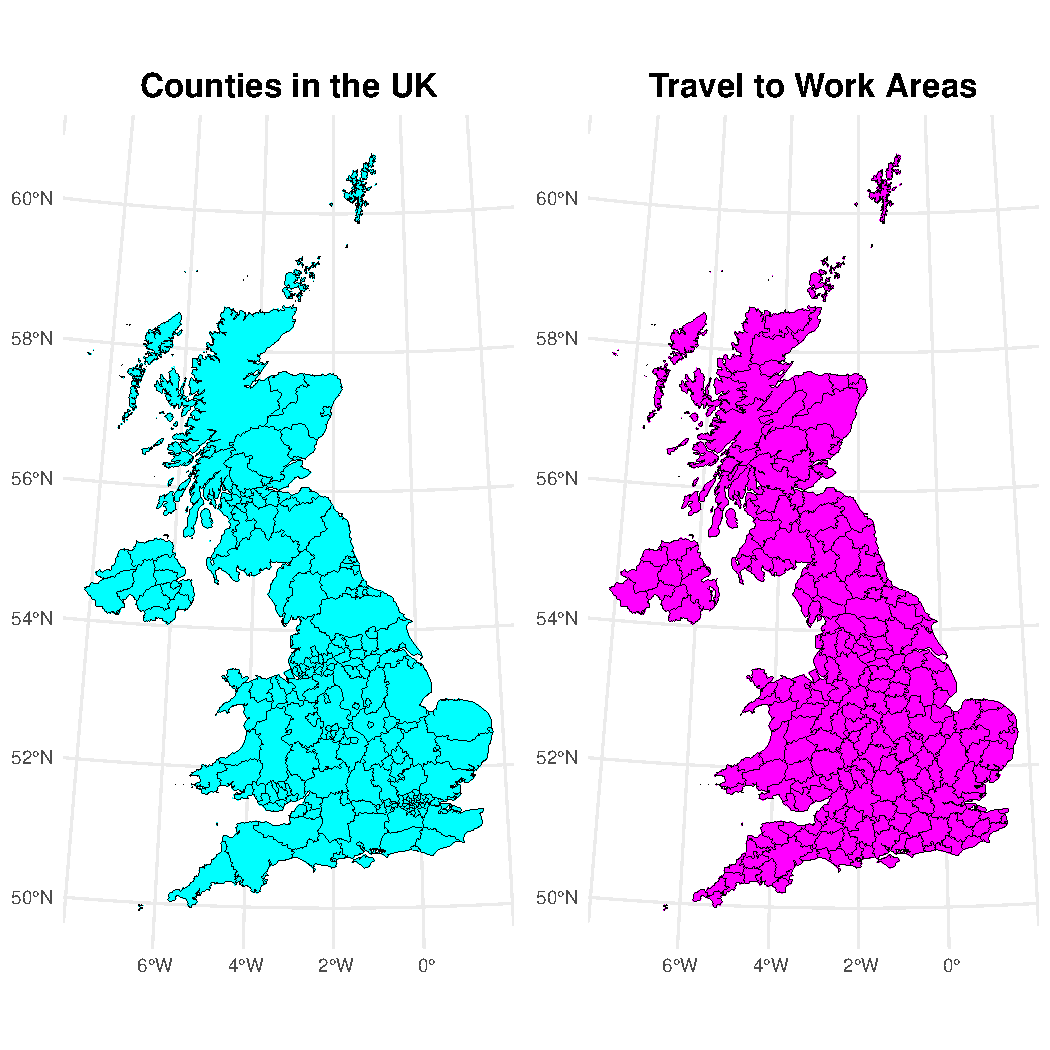
\includegraphics[width=0.55\textwidth]{images/ttwasandcounties.pdf}
    \caption{Visualization of counties and TTWAs.}
\end{figure}

\subsection*{Further Analysis of the Interlayer Network}
Further analysis of the interlayer network could provide insights into the robustness and efficiency of the UK's transport systems. This section outlines potential avenues for such analysis:

\subsubsection*{Attack Methods on Network Robustness}
Studying how different types of attacks (e.g., random failures, targeted attacks) affect the network's connectivity can reveal vulnerabilities. For example, simulating the removal of nodes or edges can help identify critical components whose failure would significantly disrupt the network.

\subsubsection*{Shortest Path Analysis Using Random Walkers}
Random walker algorithms can be employed to estimate the shortest paths within and across different transport layers. This method can highlight the efficiency of the network in terms of travel time and connectivity, providing practical insights for optimizing route planning and improving transport services.

\subsubsection*{Other Advanced Methods Studied During the Course}
Other methods such as centrality measures, community detection, and flow analysis could be applied to further dissect the network's characteristics. For instance:
\begin{itemize}
    \item \textbf{Centrality Measures:} Identifying the most influential nodes in the network based on degree centrality, betweenness centrality, or eigenvector centrality.
    \item \textbf{Community Detection:} Using algorithms like Louvain or Girvan-Newman to find clusters or communities within the network, which could correspond to functional regions or densely interconnected areas.
    \item \textbf{Flow Analysis:} Analyzing the flow of passengers or goods through the network to understand bottlenecks and optimize network performance.
\end{itemize}

These analyses can provide a deeper understanding of the transport network's dynamics and offer data-driven recommendations for enhancing its resilience and efficiency.